\documentclass[a4paper,11pt]{article}

\usepackage[utf8]{inputenc}
\usepackage[T1]{fontenc}
\usepackage{a4,graphics,amsmath,amsfonts,amsbsy,amssymb,amsthm}
\usepackage{graphicx}
\usepackage{hyperref}
\usepackage{float}
\usepackage{listings}
\usepackage{enumerate}
\usepackage{comment}
\usepackage{color}
\usepackage{accents}


\usepackage[icelandic]{babel}


\setcounter{secnumdepth}{-1}

\title{Notendasögur og Verkáætlun} \author{Matthías Páll Gissurarson  \and Sólrún Halla Einarsdóttir}

\begin{document}
\maketitle
\section{Notendasögur}
\begin{itemize}
\item Titill: Sækja gögn\\
  Lýsing: Sækja gögn um úrslit NBA-leikja af basketball-reference.com.\\
  Forgangur: 40\\
  Tími: 1 dagur\\
\item
  Titill: Geyma gögn í gagnagrunni\\
  Lýsing: Útbúa gagnagrunn sem heldur utan um gögn um úrslit leikja með skipulegum hætti svo þægilegt verði að vinna með þau.\\
  Forgangur: 40\\
  Tími: 2 dagar\\
\item
  Titill: Spá fyrir um úrslit\\
  Lýsing: Útbúa kerfi sem spáir fyrir um úrslit leiks milli gefinna liða í NBA\\
  Forgangur: 40\\
  Tími: 6 dagar\\
\item
  Titill: Vefþjónn\\
  Lýsing: Setjum upp vefþjón svo hægt sé að nota kerfið gegnum vafra\\
  Forgangur: 30\\
  Tími: 4 dagar\\
\item
  Titill: Aðgangskerfi\\
  Lýsing: Útbúa aðgangskerfi á vefþjón svo notendur geti skráð sig inn.\\
  Forgangur: 20\\
  Tími: 2 dagar\\
\item
  Titill: Halda utan um upplýsingar um notendur\\
  Lýsing: Útbúa kerfi sem heldur utan um notendanöfn, lykilorð og hversu mikið hver notandi hefur notað kerfið.\\
  Forgangur: 20\\
  Tími: 1 dagur\\
\item
  Titill: Nýta kerfið á öðrum vettvangi\\
  Lýsing: Prófa kerfið á öðrum deildum/íþróttagreinum.\\
  Forgangur: 10 \\
  Tími: 2 dagar\\
\item
  Titill: Áskrift\\
  Lýsing: Útbúa kerfi sem leyfir notendum að greiða fyrir notkun kerfis með ýmsum greiðsluleiðum. \\
  Forgangur: 10 \\
  Tími: 2 dagar\\
\item
  Titill: Rannsóknir\\
  Lýsing: Rannsaka hvað þarf í kerfið, hvað er hægt að nota til að útbúa það og hvaða gagnasöfn er hægt að hafa.\\
  Forgangur: 50\\
  Tími: 1 dagur\\
\item
  Titill: Skipulag\\
  Lýsing: Gerð notendasagna og verkáætlunnar.\\
  Forgangur: 50\\
  Tími: 1 dagur\\
\end{itemize}
\section{Verkáætlun}
Myndræna framsetningu má sjá á mynd \ref{fig:verkaetlun}
\subsection{Ítrun 0}
Notendasögur: 1. Rannsóknir 2. Skipulag\\
Áætlaður tími: 1+1 = 2 dagar
\subsection{Ítrun 1}
Notendasögur: 1. Sækja gögn 2. Geyma gögn í gagnagrunni\\
Áætlaður tími: 1+2 = 3 dagar

\subsection{Ítrun 2}
Notendasögur: 1. Spá fyrir um úrslit\\
Áætlaður tími: 6 dagar

\subsection{Ítrun 3}
Notendasögur: 1. Vefþjónn 2. Aðgangskerfi\\
Áætlaður tími: 4+2 = 6 dagar

\subsection{Ítrun 4}
Notendasögur: 1. Halda utan um upplýsingar um notendur 2. Nýta kerfið á öðrum vettvangi 3. Áskrift\\
Áætlaður tími: 1+2+2 = 5 dagar
\begin{figure}[H]
  \centering
  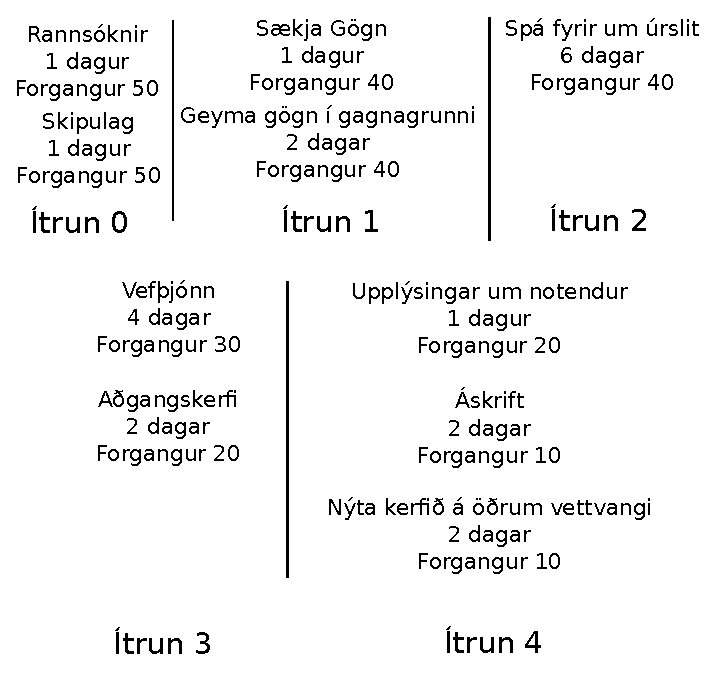
\includegraphics{verkaetlun.eps}
  \caption{Verkáætlun}
  \label{fig:verkaetlun}
\end{figure}
\end{document}